\section{系统设计}

\subsection{需求分析与模块选型}

\subsubsection{系统功能需求分析}

根据一般企事业单位对于考勤事务的管理规范,本指纹考勤系统需要实现以下几种功能,通过上位机对于下位机中指纹识别模块保存的指纹信息进行注册与删除,下位机基于前者提供的指纹数据实现基于光学识别的指纹打开签到功能。

\subsubsection{系统方案设计与选型}

根据上述系统功能需求,以树莓派4B所提供的 bcm2711 作为中央处理芯片,指纹考勤系统主要由电源供电模块,声音反馈模块,USB转TTL串口通信模块,网卡模块。
系统总体设计方案如图2.1所示。

% https://www.processon.com/v/65ec0156778cc21034664557
\begin{figure}[ht]
    \centering
    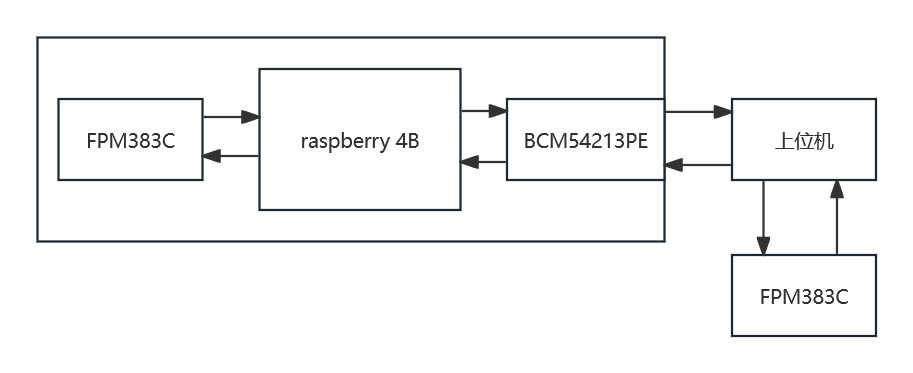
\includegraphics[width=\textwidth]{imgs/总体设计图.png}
    \caption{总体设计图}    \label{overall_design}
\end{figure}

\subsubsection{嵌入式开发板选型}

树莓派4B\ref{树莓派硬件配置说明图}使用的 bcm2711 是一种四核心64位ARM Cortex-A72架构CPU,主频高,能满足多种复杂计算需求以及满足大型程序运行需求。
树莓派4B还存在丰富而完善的接口,两个USb3.0接口,两个USB2.0接口,一个千兆网卡接口,一个HDMI接口,一个CSI接口和一个DSI接口,能够满足对于各种外设的连接需求。
树莓派4B还是树莓派第一个支持不通过 usb 直接访问网卡芯片实现网卡介入的开发板,这无形之中对于实现板载网卡驱动提供了很多帮助。

\begin{figure}[ht]
    \centering
    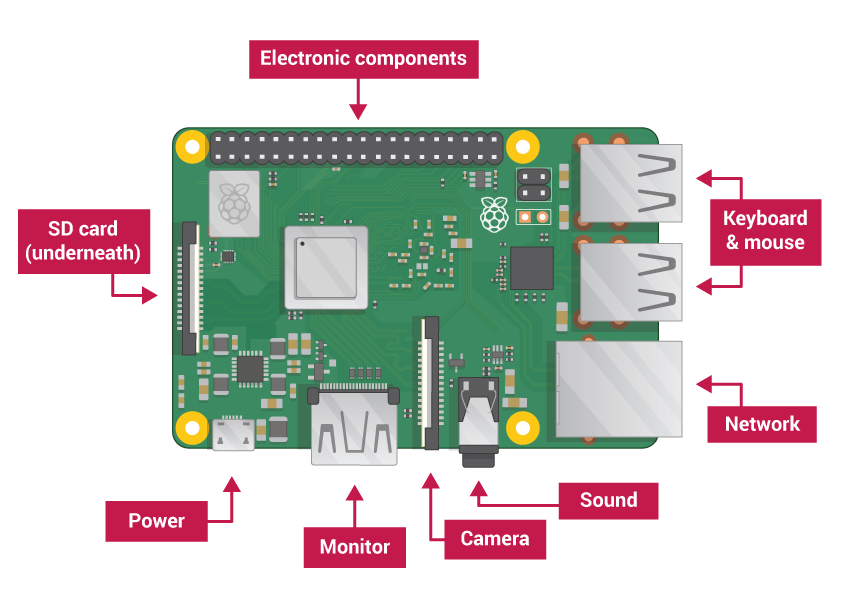
\includegraphics[width=\textwidth]{imgs/树莓派硬件配置说明图.png}
    \caption{树莓派硬件配置说明图}    \label{树莓派硬件配置说明图}
\end{figure}

\subsubsection{指纹识别模块选型}

FPM383F识别指纹模块功耗低半导体面阵传感器是一款低功耗的光学指纹识别模块,
支持对于60组光学指纹进行存储,其通过串口与中央处理器进行通信,
在串口驱动方面,基于树莓派底层寄存器UART进行调用完成对应信息的发送难度不高。

根据模组规格书,指纹模块在上电之后需要保持至少 180ms 等待才可以正常进行通信,VCC在下电之前要求设置 MCU 串口为输入高阻态,Rx 需要添加上拉电阻等需求,相对较为容易满足。

\begin{figure}[ht]
    \centering
    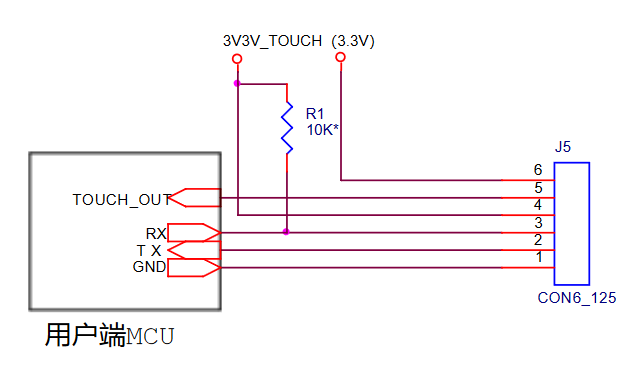
\includegraphics[scale=0.6]{imgs/FPM383C串口设备图.png}
    \caption{FPM383C串口设备图}    \label{FPM383C串口设备图}
\end{figure}


\subsubsection{通信模块选型}

    基于一般企事业单位对于考勤签到需求的需求,我计划提供多种不同的通信模块实现方便选用单位进行选择,
    其中传统基于 CH304 串口转 TTL 通信模块实现的简单串口通信主要适用于仅对于一两台设备进行支持的情况,
    而基于网卡模块间接通过网络方式拓展下位机数量的方式是主要计划实现的支持。
    针对于不同的预算管理需求,计划采用两种不同的方式实现网卡驱动,
    一种是基于 raspberry4B 板载 bcm54213PE 网卡芯片的驱动,
    另一种是基于 ENC28J60,一种基于 SPI 连接的外置 10BASE-T 以太网连接模块实现的。
    但是目前只实现了基于 BCM54213PE 网卡芯片驱动的支持。

\subsection{硬件设计}

    由于本实现相对来说比较轻量化,不太需要外部模块的支持\ref{外部模块接线图},因此只通过杜邦线进行连接,并没有画对应的板子。

    \begin{figure}[ht]
    \centering
    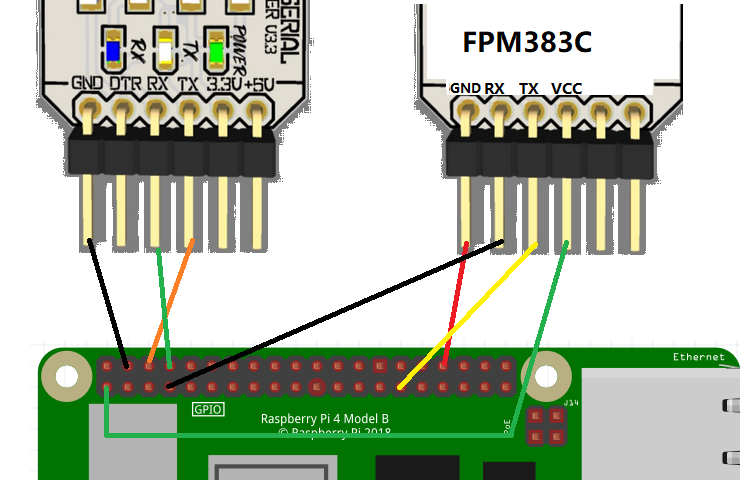
\includegraphics[scale=0.6]{imgs/接线图.png}
    \caption{外部模块接线说明图}    \label{外部模块接线图}
    \end{figure}

    \begin{itemize}
        \item 信号回返模块:
            本模块主要实现的功能在基于树莓派电信号输出,实现简单的蜂鸣功能以提醒用户当前进行的打卡已经被正确识别。
            目前有两种实现的方法,一种是基于三极管实现的长延时信号灯,另外一种是基于无源蜂鸣器实现的。
        \item 指纹采集模块:
            本模块使用了现成的串口通信指纹识别模块予以完成。
        \item 网络通信模块:
            本模块主要使用了现有的树莓派板载 PHY 芯片 BCM54213PE 实现了对应的功能,同时
            还提供了串口替代的 USB 通信方法。
    \end{itemize}

\subsection{软件设计}

    由于本研究所采用的基础嵌入式应用程序所面对的的嵌入式应用场景相对较为单一,同时也是单应用程序单地址空间的。
    \footnote{虽然底层操作系统支持使用页表进行隔离,但是在应用层面上并没有使用到虚拟页表,只是在boot的时候使用了内核页表}
    因此整体软件设计相对较为简单,主要实现难度在驱动设计层面体现,具体内容与开发过程在第三章中进行呈现。
    在嵌入式应用层面只通过循环读取 UART 串口设备驱动反馈的数据,将其分析之后的结果通过由 ArceOS 包装底层以太网驱动实现的
    UDP 包经由 RJ-45 向上位机中运行的简单管理应用程序中发送。

    在上位机中通过简易的 python 客户端程序,对于嵌入式设备中传输的 UDP 包进行分析,实现基于 Sqlite 数据库的简单指纹信息 CRUD,打卡数据 CRUD,
    与一个基于命令行实现的打卡记录查询与导出应用程序。

    \subsubsection{嵌入式软件设计}

    \begin{algorithm}[H]
        \caption{指纹识别与网络通信处理}
        \label{algorithm::fingerprint_network_comm}
        \begin{algorithmic}[1]
        \While{true} \Comment{无限循环处理事件}
            \State \Call{LogDebug}{"===================================="}
            \State \textbf{try} \Call{ReceiveData}{$socket, \& buf$}
            \If{\Call{Receive}{$socket, \& buf$} = Ok$(size, addr)$}
                \State $buf \gets [0; 1024]$ \Comment{重置缓冲区}
            \ElsIf{\textbf{error} = WouldBlock}
                \State \textbf{continue}
            \Else
                \State \Call{LogDebug}{\textbf{error}}
            \EndIf
            \State \Call{LogDebug}{"AAA"}
        
            \For{$item$ \textbf{in} $fpm383c::SEARCH\_FINGERPRINT\_MATCH\_START$}
                \State \Call{Write}{$serial, item$}
            \EndFor
            \State \Call{Delay}{10}
            \State \Call{GetFrame}{$serial$}
            
            \For{$item$ \textbf{in} $fpm383c::CHECK\_FINGERPRINT\_MATCH\_RESULT$}
                \State \Call{Write}{$serial, item$}
            \EndFor
        
            \If{$frame \gets$ \Call{GetFrame}{$serial$}}
                \State \Call{Assert}{$frame$, CmdType::CheckMatchFingerprint}
                \State $data \gets$ \Call{GetAllUsersData}{$frame$}
                \State \Call{LogDebug}{"data: $data$"}
                \State $data \gets$ \Call{GetUserData}{$frame, 0, 2$}
                
                \If{\Call{Any}{$data, \neq 0$}}
                    \State \textbf{initialize} $sign\_in\_buf \gets [0x46, 0x69, \ldots, 0x20]$
                    \State \Call{SetSignInData}{$frame, sign\_in\_buf$}
                    \State \Call{SendTo}{$local\_socket, sign\_in\_buf, TARGET\_IP, TARGET\_PORT$}
                    \For{$item$ \textbf{in} $fpm383c::SLICE\_OF\_GREENFLASHING\_MODE$}
                        \State \Call{Write}{$serial, item$}
                    \EndFor
                \Else
                    \For{$item$ \textbf{in} $fpm383c::SLICE\_OF\_REDFLASHING\_MODE$}
                        \State \Call{Write}{$serial, item$}
                    \EndFor
                \EndIf
                \State \Call{GetFrame}{$serial$}
                \State \Call{Delay}{10}
            \EndIf
        \EndWhile
        \end{algorithmic}
        \end{algorithm}
        

    \subsubsection{数据库设计}

    \subsubsection{功能说明}

    \begin{description}
        \item[指纹注册] 由上位机中自动完成指纹注册,通过上传命令,获取对应ID的指纹特征信息并以UDP包的形式下发到下位机中的指纹模块。
        
        指纹注册功能主要在上位机中完成,这主要是考量到在 HR 处实现人事登记等操作
        更加合乎一般企业的考勤流程。
        
        通过 0x0118 命令\ref{uart::auto-register},实现自动注册功能,该命令会自动完成采图、提取、拼接、保存等操作,
        该部分通过分析返回包中的ID和注册进度进行操作,在注册进度达到 0x64 时终止注册流程。

        \begin{table}[htbp]
            \resizebox{\textwidth}{!}{%
                \begin{tabular}{|l|l|l|l|l|l|l|l|}
                \hline
                \multicolumn{1}{|c|}{校验密码} & CMD类型 & CMD号 & 等待手指 & 按压次数 & ID\_H & ID\_L & 校验和  \\ \hline
                0x00 0x00 0x00 0x00        & 0x01  & 0x18 & 0x01 & 0x06 & 0xFF  & 0xFF  & 0xE2 \\ \hline
                \end{tabular}
            }
            \caption{自动注册命令用户层帧} \label{uart::auto-register}
        \end{table}

        在注册完成之后,通过上载命令\ref{uart::upload-info},向指纹模块获取特定 ID 号的指纹特征信息长度,
        然后再通过 \ref{uart::upload-data} 命令,从指纹模块获取对应分片的指纹特征信息。
        在将信息存储到数据库的同时,还通过 UDP 包的形式,将对应的数据发送到树莓派,树莓派再将对应指纹特征信息
        下载到树莓派对应的指纹模块上,由此完成了一次标准的指纹注册功能。

        \begin{table}[htbp]
            \resizebox{\textwidth}{!}{%
                \begin{tabular}{|l|l|l|l|l|l|}
                \hline
                \multicolumn{1}{|c|}{校验密码} & CMD类型 & CMD号 & ID\_H & ID\_L & 校验和  \\ \hline
                0x00 0x00 0x00 0x00        & 0x01  & 0x53 & 0x00  & 0x01  & 0xAB \\ \hline
                \end{tabular}
            } \caption{获取上传信息命令用户层帧} \label{uart::upload-info}
        \end{table}

        \begin{table}[htbp]
            \resizebox{\textwidth}{!}{%
            \begin{tabular}{|l|l|l|l|l|l|l|l|}
                \hline
                \multicolumn{1}{|c|}{校验密码} & CMD类型 & CMD号 & ID\_H & ID\_L & NUM\_H & NUM\_L & 校验和  \\ \hline
                0x00 0x00 0x00 0x00        & 0x01  & 0x51 & 0xFF  & 0xFF  & 0x00   & 0x00   & 0xAC \\ \hline
                \end{tabular}
            } \caption{获取指纹特征命令用户层帧} \label{uart::upload-data}
        \end{table}

        \item[指纹删除] 在上位机中完成指纹删除操作,通过下行 Udp 包,删除指纹模块中对应 ID 的指纹特征信息。
        
        指纹删除功能主要在上位机中完成,在出现指纹出现问题的时候,由 HR 执行运行函数,自动化删除数据库中员工对应的指纹特征编号,
        同时将删除指纹特征编号的命令通过下面的指令\ref{指纹特征清除}经由树莓派下发到指纹终端,根据不同的需求,在下面的帧中配置不同的格式。

        \begin{table}[ht]
            \resizebox{\textwidth}{!}{%
                \begin{tabular}{|l|l|l|l|l|l|l|}
                \hline
                \multicolumn{1}{|c|}{校验密码} & CMD类型 & CMD号 & CL\_FLAG & ID\_H & ID\_L & 校验和  \\ \hline
                0x00 0x00 0x00 0x00        & 0x01  & 0x51 & 03       & 0xFF  & 0xFF  & 0xAC \\ \hline
                \end{tabular} 
            } \caption{指纹特征清除} \label{指纹特征清除}
        \end{table}

        \item[指纹考勤登记] 在下位机从属指纹模块中完成基于指纹的考勤实现。
        
        下位机会循环的向指纹模块询问指纹能否匹配\ref{询问是否匹配},并按照匹配应答包\ref{匹配应答包}格式返回对应结果,
        根据对应的匹配分数以及是否完成匹配。

        当当前指纹被实际判断匹配成功,对应的数据就会被放在下面的帧结构中,再通过 UdpSocket 发送到上位机的 Socket,
        上位机中利用 Python Socket 对于 5555 端口进行长期监听,对所有监听到的数据包进行匹配,当前后帧结构一致的情况下
        将其中包含的 ID 按照 sqlite 的规定插入到对应表中
        \footnote{sqlite中有一种名为 CURRENT\_TIMESTAMP 的默认属性,会默认将插入项的时间作为一个元素一起插入}。

        \begin{table}[htbp]
            \resizebox{\textwidth}{!}{%
                \begin{tabular}{|l|l|l|l|}
                \hline
                \multicolumn{1}{|c|}{校验密码} & CMD类型 & CMD号    & 校验和  \\ \hline
                0x00 0x00 0x00 0x00        & 0x01  & 0x21 / 0x22 & 0xAC \\ \hline
                \end{tabular}
            }  \caption{询问是否匹配,查询匹配结果} \label{询问是否匹配}
        \end{table}

        \begin{table}[htbp]
            \resizebox{\textwidth}{!}{%
                \begin{tabular}{|l|l|l|l|l|l|l|l|}
                \hline
                \multicolumn{1}{|c|}{校验密码} & CMD类型 & CMD号 & 错误码                 & 匹配结果      & 匹配分数      & 匹配ID      & 校验和  \\ \hline
                0 0 0 0        & 0x01  & 0x51 & 0 0 0 0 & 0x00 0x01 & 0x27 0x0F & 0x00 0x03 & 0xAC \\ \hline
                \end{tabular} 
            }  \caption{匹配应答包格式} \label{匹配应答包}
        \end{table}

        \item[考勤记录读取] 根据一般企事业单位的考勤系统的历史发展来看,读取员工考勤记录属于考勤系统的必备功能。
        
        本功能主要实现在上位机处,由上位机调用函数对于原先保存在sqlite中的考勤打卡表与员工-指纹特征对应表进行自动关联,并且
        基于一定的逻辑分析打印出员工的详细打卡数据与月度打卡数据。
    \end{description}
      

